
\section{Avro}
\label{section:avro}

Αποτελεί μία μορφή αποθήκευσης πληροφορίας που, λόγω της υλοποίησης του, παράγει αρχεία
πολύ μικρότερου μεγέθους από ότι θα αναμέναμε σε άλλου είδους μορφές αρχείων. Αναπτύχθηκε αρχικά για
την αποθήκευση και τη μετάδοση πληροφορίας εντός του framework Apache Hadoop, αλλά έκτοτε
έχει χρήση και σε πλήθος άλλων εφαρμογών. Διαθέτει διεπαφές (API) που επιτρέπουν την ενσωμάτωση της τεχνολογίας αυτής σε
προγμάμματα γραμμένα σε πλήθος γλωσσών, μερικές εκ των οποίων είναι οι Java, C/C++/C\#, Python, PHP, Ruby, Rust και JavaScript.

Η βασικότερη διαφορά μεταξύ αρχείων avro και άλλων αρχείων αποθήκευσης πληροφορίας, όπως είναι τα JSON αρχεία,
που αποτελούν τον πιο διαδεδομένο τρόπο αποθήκευσης στο χώρο του διαδικτύου, είναι το γεγονός
ότι διαθέτουν το schema των δεδομένων (data schema definition) που περιέχουν. Ξέροντας τη μορφή της προς αποθήκευση πληροφορίας
καταφέρνουν να γλιτώσουν χώρο στο τελικό προϊόν. Αυτό σε συνδύασμό με το γεγονός ότι η πληροφορία αποθηκεύεται
συμπιεσμένη σε δυαδική μορφή (binary format) την καθιστά αρκετά σημαντική σε περιπτώσεις που έχουμε μεγάλο πλήθος πληροφορίας
που θέλουμε να αποθηκεύσουμε.

Τα βασικότερα πλεονεκτήματα του παρατίθενται στη συνέχεια ενώ η δομή ενός τέτοιου αρχείου φαίνεται στο \autoref{fig:avro_file_format}:

\begin{itemize}
	\item Είναι χρήσιμος για την μετάδοση πληροφορίας, καθώς η αποθηκευμένη πληροφορία είναι
		αρκετά συμπυκνωμένη.
	\item Επιτρέπει την τροποποίηση και εξέλιξη του σχήματος των δεδομένων (schema evolution), δίνοντας
		τη δυνατότητα για αλλαγές και data migration που πολλές φορές καθίστανται επιτακτικά 
		στη διάρκεια ζωής ενός προγράμματος που συνεχώς εξελίσσεται.
	\item Διαθέτει πλήθος τύπων δεδομένων απλών (primitive) και σύνθετων (complex) που μπορούν να χρησιμοποιηθούν
		\begin{itemize}
			\item Primitive: boolean, int, long, float, double, bytes, string
			\item Complex: record, enum, array, map, fixed, union 
		\end{itemize}
	\item Το schema εμπεριέχεται σε κάθε αρχείο. Κάνοντας χρήση αυτού, κάθε χρήστης που έχει
		πρόσβαση σε ένα τέτοιο αρχείο μπορεί να διαβάσει τα περιεχόμενα του (εξαρχής binary, μη αναγνώσιμων από τον άνθρωπο)
		χωρίς να ξέρει από πριν τη μορφή της πληροφορίας. 
\end{itemize}


\begin{figure}[!ht]
	\centering
	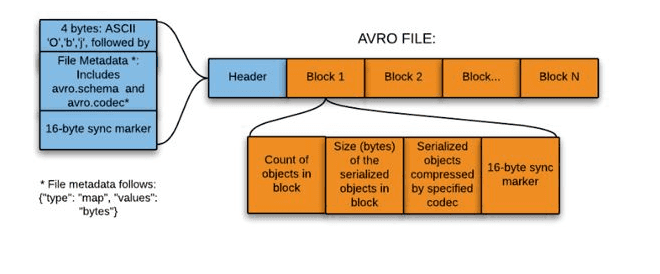
\includegraphics[width=0.7\textwidth]{./images/chapter2/avro_file_format.png}
	\caption[Δομή ενός avro αρχείου]{Δομή ενός avro αρχείου}
	\label{fig:avro_file_format}
\end{figure}